\section{Durchführung}
\label{sec:Durchführung}
\subsection{Verwendete Elemente und grundlegender Aufbau}
Zunächst ist eine Spannungsquelle vorhanden, die zwei Spannungen erzeugen und augeben kann. 
Die Spannung kann dabei über Drehknöpfe eingestellt werden.
Da bei einem der beiden Ausgänge allerdings die vom Generator angezeigte Spannung nicht stimmt, steht zusätzlich ein Voltmeter zur Verfügung. 
Dieses wird durch die vorhandenen Kabel mit Bananensteckern an den entsprechenden Ausgang verbunden, um die Spannung überprüfen zu können.
Der positive Ausgang der ersten Spannung des Generators wird mit dem Eingang $V_b$ des ebenfalls vorhandenen Breadboards verbunden.
Der negative Ausgang der ersten Spannung wird sowohl mit dem Anschluss für die Masse auf dem Breadboard als auch mit dem positiven Ausgang der zweiten Spannung am Generator verbunden.
Der negative Ausgang der zweiten Spannung wird wiederum mit dem Anschluss $V_a$ verbunden. So ist diese Spannung invertiert bzw. negativ. \textbf{PRUEFEN OB SO ODER ANDERS HERUM}
Am Generator wird nunr bei beiden Spannungen jeweils $\qty{15}{\volt}$ eingestellt. 
So wird die Versorgungsspannung für den Operationsverstärker erzeugt.
\\ 
Außerdem wird ein Signalgenerator verwendet, welcher Sinus-, Dreiecks- und Rechteckspannungen ausgeben kann, wobei Frequenz und Amplitude frei einstellbar sind.
Mit einem entsprechenden Kabel, kann dessen ausgang mit dem Eingang $V_c$ und der Masse des Breadboards verbunden werden. 
Dadurch wird auch das Eingangssignal für den Operationsverstärker generiert.
\\
Durch ein T-Stück und ein BNC-Kabel wird der Ausgang des Signalgenerators auch an den einen Eingang eines Zwei-Kanal-Oszilloskops angeschlossen. 
Der andere Eingang des Oszilloskops wird über einen Adapter an das Breadboard angeschlossen. 
So kann bei der Durchführung Ein- und Ausgangssignal am Oszilloskop vermessen werden. 
\\
Auf dem Breadbord können so die in \autoref{sec:schaltungen} beschriebenen Schaltungen aufgebaut werden. 
Dazu sind verschiedene Operationsverstärker der Typen LM741, LM358 und TL072 vorhanden.
Allerdings wird hier nur ein Operationsverstärker des Typs LM741 verwendet.
Außerdem stehen mehrere \textbf{KABELTYP VON DEN KLEINEN KABELN} sowie verschiedene Widerstände und Kondensatoren zur Verfügung.
In \autoref{fig:aufbau} ist der gesamte so eben beschriebene Aufbau zu sehen. 
\begin{figure}
  \centering
  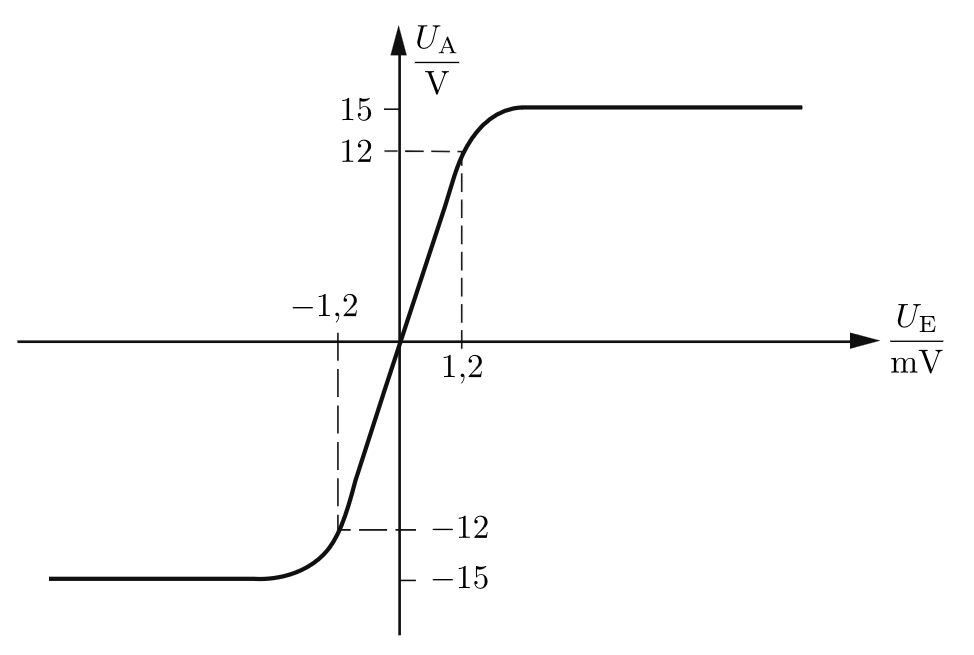
\includegraphics[width=0.7\textwidth]{content/images/kennlinie.png}
  \caption{\textbf{NOCH EINFUEGEN!}.}
  \label{fig:aufbau}
\end{figure}


\subsection{Untersuchung des Linearverstärkers}
Zur Untersuchung des invertierenden Linearverstärkers wird dieser zunächst auf dem Breadboard wie in \autoref{fig:schalt1} zu sehen Aufgebaut. 
\textbf{WAS WIRD WIE VERBUNDEN}
\\
Nun können für vier verschiedene Verstärkungen bzw. Verhältnisse der eingesetzten Widerstände die Verstärkung abhängig von der Frequenz vermessen werden. 
Dazu wird zunächst am Signalgenerator eine feste Amplitude eingestellt. 
Anschließen wird die Frequenz bei $\qty{1}{\hertz}$ startend über mehrere Dekaden in exponentiell größer werdenden Schritten erhöht. 
Bei jedem Schritt wird mit dem Cursor am Oszilloskop dann sowohl die Amplitude des Ausgangssignals als auch der zeitliche Abstand zwischen den beiden Signalen gemessen.
Letzteres gelingt, indem von Maximum des Eingangssignals zu Maximum des Ausgangssignals gemessen wird. 
Daraus kann dann der Phasenversatz bestimmt werden. 
Dies wird für die vier Verhähltnisse von Widerständen durchgeführt, wie sie in \autoref{tab:widerstaende} dargestellt sind.
Außerdem ist auch die jeweils eingestellte Amplitude am Signalgenerator eingetragen.
\begin{table}
  \centering
  \caption{\textbf{TABELLE NOCH AUSFUELLEN!}}
  \label{tab:tabelle}
  \sisetup{table-format=1.1, per-mode=reciprocal}
  \begin{tblr}{
      colspec = {S[table-format=3.0] S[table-format=2.1] S},
      row{1} = {guard, mode=math},
      %vline{4} = {2}{-}{text=\clap{$\pm$}},
    }
    \toprule
    \mathrm{Messdurchgang}&R_1 \mathbin{/} \unit{\ohm} & R_2 \mathbin{/} \unit{\ohm} & U_{\mathrm{e,max}} \\
    \midrule
    1 & 0 & 0 & 0 \\
    2 & 0 & 0 & 0 \\
    3 & 0 & 0 & 0 \\
    4 & 0 & 0 & 0 \\
    \bottomrule
  \end{tblr}
\end{table}


\subsection{Untersuchung des Integrators und des Differenzierers}


\subsection{Untersuchung des Schmitt-Triggers}